% Options for packages loaded elsewhere
\PassOptionsToPackage{unicode}{hyperref}
\PassOptionsToPackage{hyphens}{url}
\documentclass[
  ignorenonframetext,
]{beamer}
\newif\ifbibliography
\usepackage{pgfpages}
\setbeamertemplate{caption}[numbered]
\setbeamertemplate{caption label separator}{: }
\setbeamercolor{caption name}{fg=normal text.fg}
\beamertemplatenavigationsymbolsempty
% remove section numbering
\setbeamertemplate{part page}{
  \centering
  \begin{beamercolorbox}[sep=16pt,center]{part title}
    \usebeamerfont{part title}\insertpart\par
  \end{beamercolorbox}
}
\setbeamertemplate{section page}{
  \centering
  \begin{beamercolorbox}[sep=12pt,center]{section title}
    \usebeamerfont{section title}\insertsection\par
  \end{beamercolorbox}
}
\setbeamertemplate{subsection page}{
  \centering
  \begin{beamercolorbox}[sep=8pt,center]{subsection title}
    \usebeamerfont{subsection title}\insertsubsection\par
  \end{beamercolorbox}
}
% Prevent slide breaks in the middle of a paragraph
\widowpenalties 1 10000
\raggedbottom
\AtBeginPart{
  \frame{\partpage}
}
\AtBeginSection{
  \ifbibliography
  \else
    \frame{\sectionpage}
  \fi
}
\AtBeginSubsection{
  \frame{\subsectionpage}
}
\usepackage{iftex}
\ifPDFTeX
  \usepackage[T1]{fontenc}
  \usepackage[utf8]{inputenc}
  \usepackage{textcomp} % provide euro and other symbols
\else % if luatex or xetex
  \usepackage{unicode-math} % this also loads fontspec
  \defaultfontfeatures{Scale=MatchLowercase}
  \defaultfontfeatures[\rmfamily]{Ligatures=TeX,Scale=1}
\fi
\usepackage{lmodern}
\ifPDFTeX\else
  % xetex/luatex font selection
\fi
% Use upquote if available, for straight quotes in verbatim environments
\IfFileExists{upquote.sty}{\usepackage{upquote}}{}
\IfFileExists{microtype.sty}{% use microtype if available
  \usepackage[]{microtype}
  \UseMicrotypeSet[protrusion]{basicmath} % disable protrusion for tt fonts
}{}
\makeatletter
\@ifundefined{KOMAClassName}{% if non-KOMA class
  \IfFileExists{parskip.sty}{%
    \usepackage{parskip}
  }{% else
    \setlength{\parindent}{0pt}
    \setlength{\parskip}{6pt plus 2pt minus 1pt}}
}{% if KOMA class
  \KOMAoptions{parskip=half}}
\makeatother
\usepackage{longtable,booktabs,array}
\newcounter{none} % for unnumbered tables
\usepackage{calc} % for calculating minipage widths
\usepackage{caption}
% Make caption package work with longtable
\makeatletter
\def\fnum@table{\tablename~\thetable}
\makeatother
\setlength{\emergencystretch}{3em} % prevent overfull lines
\providecommand{\tightlist}{%
  \setlength{\itemsep}{0pt}\setlength{\parskip}{0pt}}
\usepackage{bookmark}
\IfFileExists{xurl.sty}{\usepackage{xurl}}{} % add URL line breaks if available
\urlstyle{same}
\hypersetup{
  hidelinks,
  pdfcreator={LaTeX via pandoc}}

\author{\texorpdfstring{}{}}
\date{}

\begin{document}

\begin{frame}[fragile]{Hypothesis Evidence Landscape and Temporal
Dynamics \label{sec:hypothesis_results}}
\protect\phantomsection\label{hypothesis-evidence-landscape-and-temporal-dynamics}
The LLM-based extraction pipeline produced a total of 2,795 assertions
across the eight tracked hypotheses, drawn from the full corpus of
\(N = 849\) papers. The distribution of assertion types and the
resulting citation-weighted scores reveal a differentiated evidence
landscape (Figure \ref{fig:hypothesis_dashboard}):

{\def\LTcaptype{none} % do not increment counter
\begin{longtable}[]{@{}
  >{\raggedright\arraybackslash}p{(\linewidth - 12\tabcolsep) * \real{0.1429}}
  >{\raggedright\arraybackslash}p{(\linewidth - 12\tabcolsep) * \real{0.1429}}
  >{\raggedright\arraybackslash}p{(\linewidth - 12\tabcolsep) * \real{0.1429}}
  >{\raggedright\arraybackslash}p{(\linewidth - 12\tabcolsep) * \real{0.1429}}
  >{\raggedright\arraybackslash}p{(\linewidth - 12\tabcolsep) * \real{0.1429}}
  >{\raggedright\arraybackslash}p{(\linewidth - 12\tabcolsep) * \real{0.1429}}
  >{\raggedright\arraybackslash}p{(\linewidth - 12\tabcolsep) * \real{0.1429}}@{}}
\toprule\noalign{}
\begin{minipage}[b]{\linewidth}\raggedright
Hypothesis
\end{minipage} & \begin{minipage}[b]{\linewidth}\raggedright
Score
\end{minipage} & \begin{minipage}[b]{\linewidth}\raggedright
Supports
\end{minipage} & \begin{minipage}[b]{\linewidth}\raggedright
Neutral
\end{minipage} & \begin{minipage}[b]{\linewidth}\raggedright
Contradicts
\end{minipage} & \begin{minipage}[b]{\linewidth}\raggedright
Total
\end{minipage} & \begin{minipage}[b]{\linewidth}\raggedright
Character
\end{minipage} \\
\midrule\noalign{}
\endhead
H4: Predictive Coding & \(+0.92\) & 677 & 115 & 1 & 793 & Strong
consensus \\
H5: Scalability & \(+0.68\) & 126 & 95 & 0 & 221 & Strong consensus \\
H8: Language AIF & \(+0.48\) & 39 & 70 & 0 & 109 & Moderate, growing \\
H6: Clinical Utility & \(+0.42\) & 14 & 21 & 0 & 35 & Moderate,
emerging \\
H7: Morphogenesis & \(+0.40\) & 16 & 45 & 0 & 61 & Moderate, emerging \\
H1: FEP Universality & \(+0.38\) & 250 & 546 & 1 & 797 & Broad but
diffuse \\
H2: AIF Optimality & \(+0.24\) & 142 & 477 & 15 & 634 & Weakly
contested \\
H3: Markov Blanket Realism & \(+0.22\) & 11 & 130 & 4 & 145 &
Contested \\
\bottomrule\noalign{}
\end{longtable}
}

\begin{figure}[htbp]
\centering
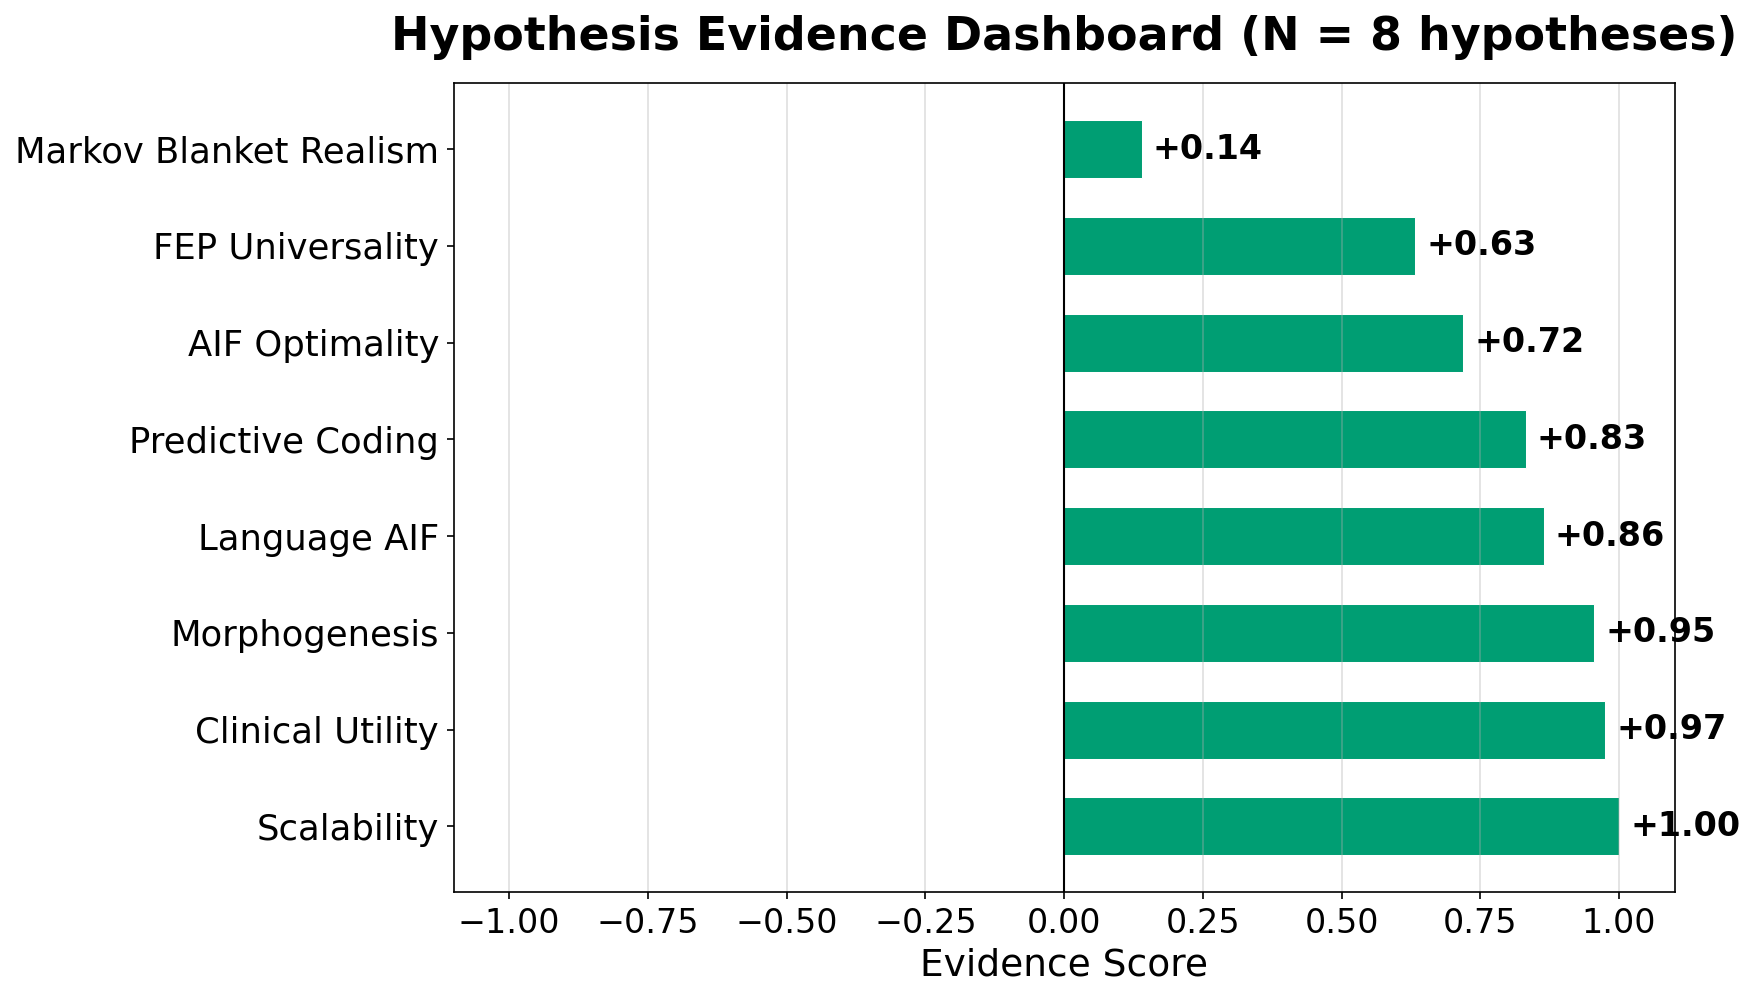
\includegraphics[width=0.9\textwidth]{../figures/hypothesis_dashboard.png}
\caption{Hypothesis scoring dashboard showing citation-weighted evidence scores ($[-1, +1]$) for the eight tracked hypotheses, sorted descending by consensus strength. Predominantly positive scores reflect both genuine empirical support and systematic positive biases from publication selection and linguistic framing (see \S\ref{sec:pub_bias}).}
\label{fig:hypothesis_dashboard}
\end{figure}

\begin{block}{Interpretation of Evidence Profiles}
\protect\phantomsection\label{interpretation-of-evidence-profiles}
The eight hypotheses cluster into three distinct tiers. The
\textbf{consensus tier} (H4, H5) comprises hypotheses with strong
positive scores (\(> 0.5\)) and minimal contradicting assertions.
Predictive coding (H4), the most extensively assessed hypothesis with
793 assertions and a score of \(+0.92\), has accumulated overwhelmingly
supportive evidence since the 1970s, reflecting the deep empirical
grounding of hierarchical prediction error models in neuroscience.
Scalability (H5) shows a similarly strong positive trajectory
(\(+0.68\)) that accelerated after 2017 as deep active inference
architectures emerged.

The \textbf{moderate tier} (H6, H7, H8) comprises hypotheses with
positive scores in the \(0.4\)--\(0.5\) range. Language AIF (H8) leads
this tier with 109 assertions and a score of \(+0.48\), reflecting
recent breakthroughs coupling active inference to large language models.
Clinical utility (H6) has the smallest evidence base (35 assertions) but
shows a temporally increasing trend, consistent with the recent growth
of computational psychiatry applications. Morphogenesis (H7) shows
moderate support (\(+0.40\)), reflecting its status as an active
research frontier where theoretical proposals outpace empirical
validation.

The \textbf{diffuse or contested tier} (H1, H2, H3) is the most
diagnostically informative for understanding the field's intellectual
maturation. FEP universality (H1), despite generating one of the largest
raw evidence bases (797 assertions), achieves a score of only
\(+0.38\)---the majority of assessments are neutral, indicating that
researchers frequently \emph{invoke} the FEP without explicitly testing
its universality claim. This finding dovetails with the falsifiability
critique leveled by Colombo and Seri`es \citep{colombo2021free}: if the
FEP can be applied to any self-organizing system without generating
testable predictions that distinguish it from alternative frameworks,
neutral citations (invocations rather than tests) are exactly what one
would expect to dominate the literature. AIF optimality (H2) exhibits
the largest volume of contradicting evidence (15 assertions), suggesting
that as the field has transitioned from theory to empirical application,
absolute optimality claims have undergone increasingly stringent
critical scrutiny. Markov blanket realism (H3) has the smallest evidence
base (145 assertions) with a score of \(+0.22\) and 4 contradicting
assertions---empirically capturing the ongoing philosophical debate
between those who treat Markov blankets as real thermodynamic boundaries
("Friston blankets") and those who argue they are purely instrumental
statistical tools ("Pearl blankets") \citep{bruineberg2022emperor}. The
contested score for H3 directly reflects this unresolved ontological
tension in the field.
\end{block}

\begin{block}{Temporal Dynamics of Evidence Accumulation}
\protect\phantomsection\label{temporal-dynamics-of-evidence-accumulation}
The cumulative evidence timeline (Figure \ref{fig:evidence_timeline})
reveals three temporal patterns. First, \textbf{early convergence}: H4
(predictive coding) reached positive territory in the late 1990s
following the publication of Rao and Ballard's foundational predictive
coding model \citep{rao1999predictive} and has maintained a high score
since, reflecting the mature empirical base in cognitive neuroscience.
Second, \textbf{recent acceleration}: H5 (scalability) and H6 (clinical
utility) show steep upward trends after 2017, tracking the emergence of
deep active inference tools and computational psychiatry applications.
The H5 trajectory is particularly striking: AXIOM \citep{heins2025axiom}
demonstrates that principled object-centric world models under the AIF
framework can outperform state-of-the-art deep RL agents on standard
benchmarks, directly addressing the scalability challenge that has
historically been the strongest argument against AIF as a practical
framework. Third, \textbf{persistent contestation}: H3 (Markov blanket
realism) has maintained a lower score since 2018, with supporting papers
partially offset by targeted critiques.

\begin{figure}[htbp]
\centering
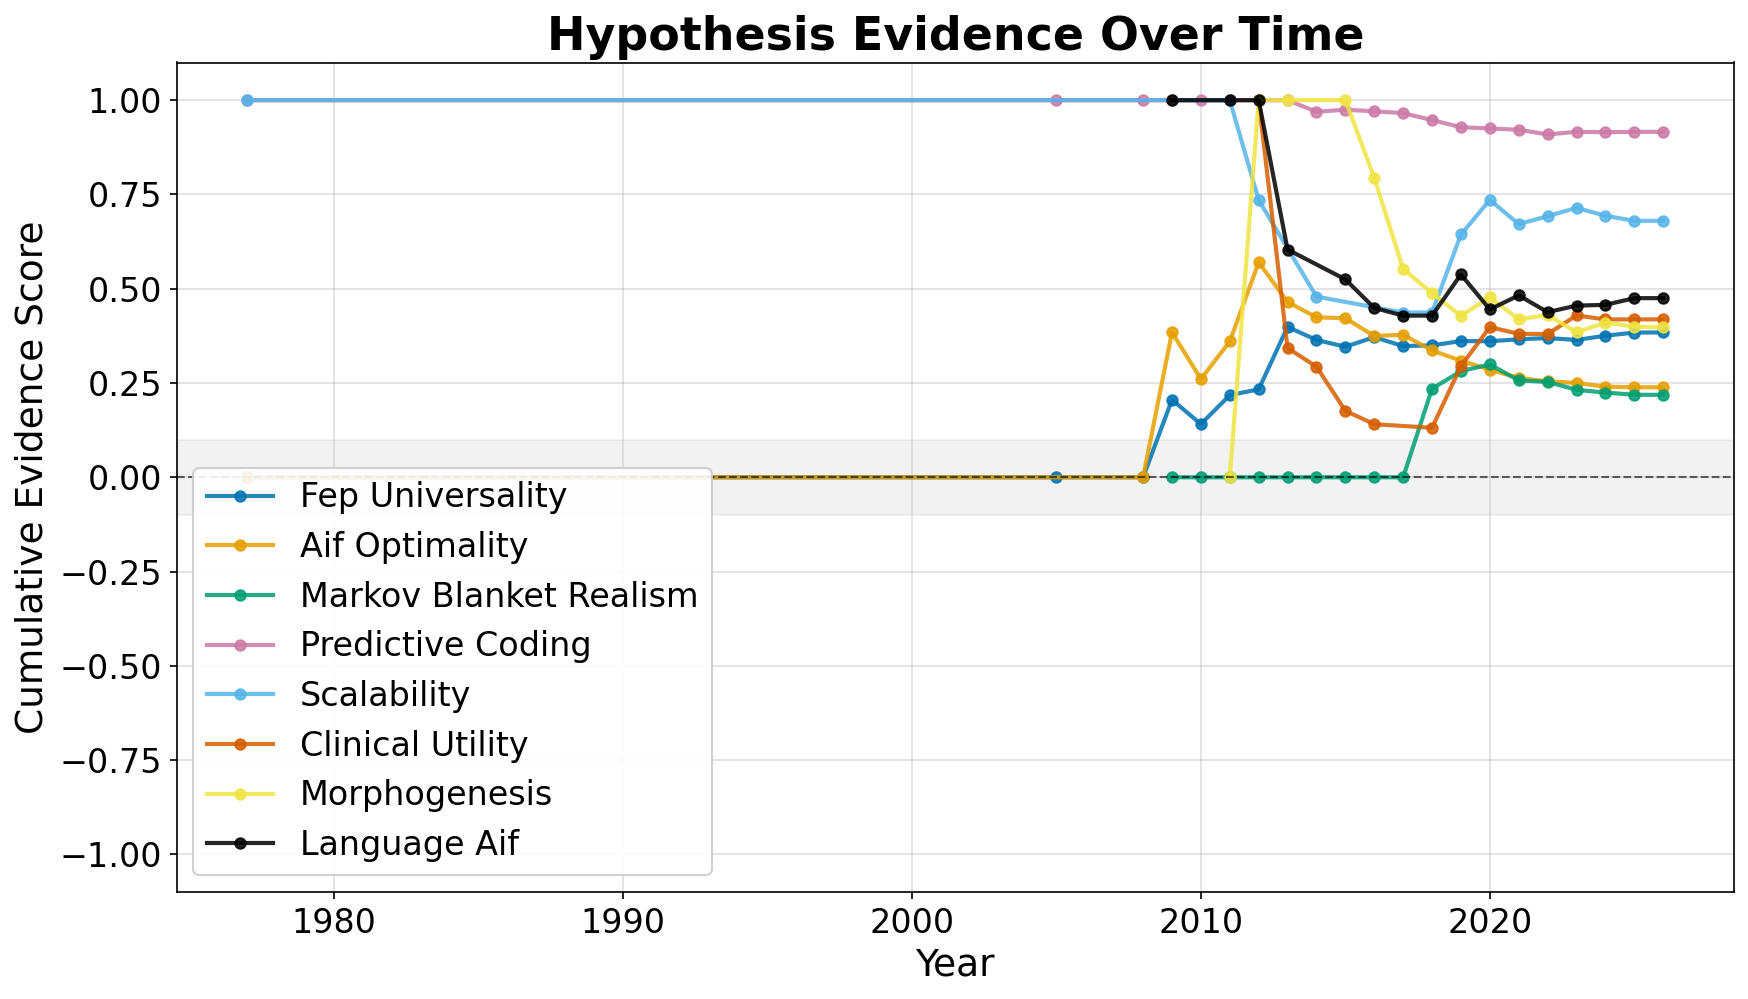
\includegraphics[width=0.9\textwidth]{../figures/evidence_timeline.png}
\caption{Temporal evolution of cumulative citation-weighted evidence scores by hypothesis (2005--2026). Divergent trajectories around the shaded neutral boundary $(\pm 0.1)$ reveal which hypotheses are gaining or losing support over time. H4 (predictive coding) stabilized early; H5 (scalability) accelerated post-2017.}
\label{fig:evidence_timeline}
\end{figure}
\end{block}

\begin{block}{Assertion Composition and Distribution}
\protect\phantomsection\label{assertion-composition-and-distribution}
The per-hypothesis composition of assertions (Figure
\ref{fig:assertion_breakdown}) and the multi-panel summary (Figure
\ref{fig:assertion_summary}) provide complementary views of the
extraction results.

\begin{figure}[htbp]
\centering
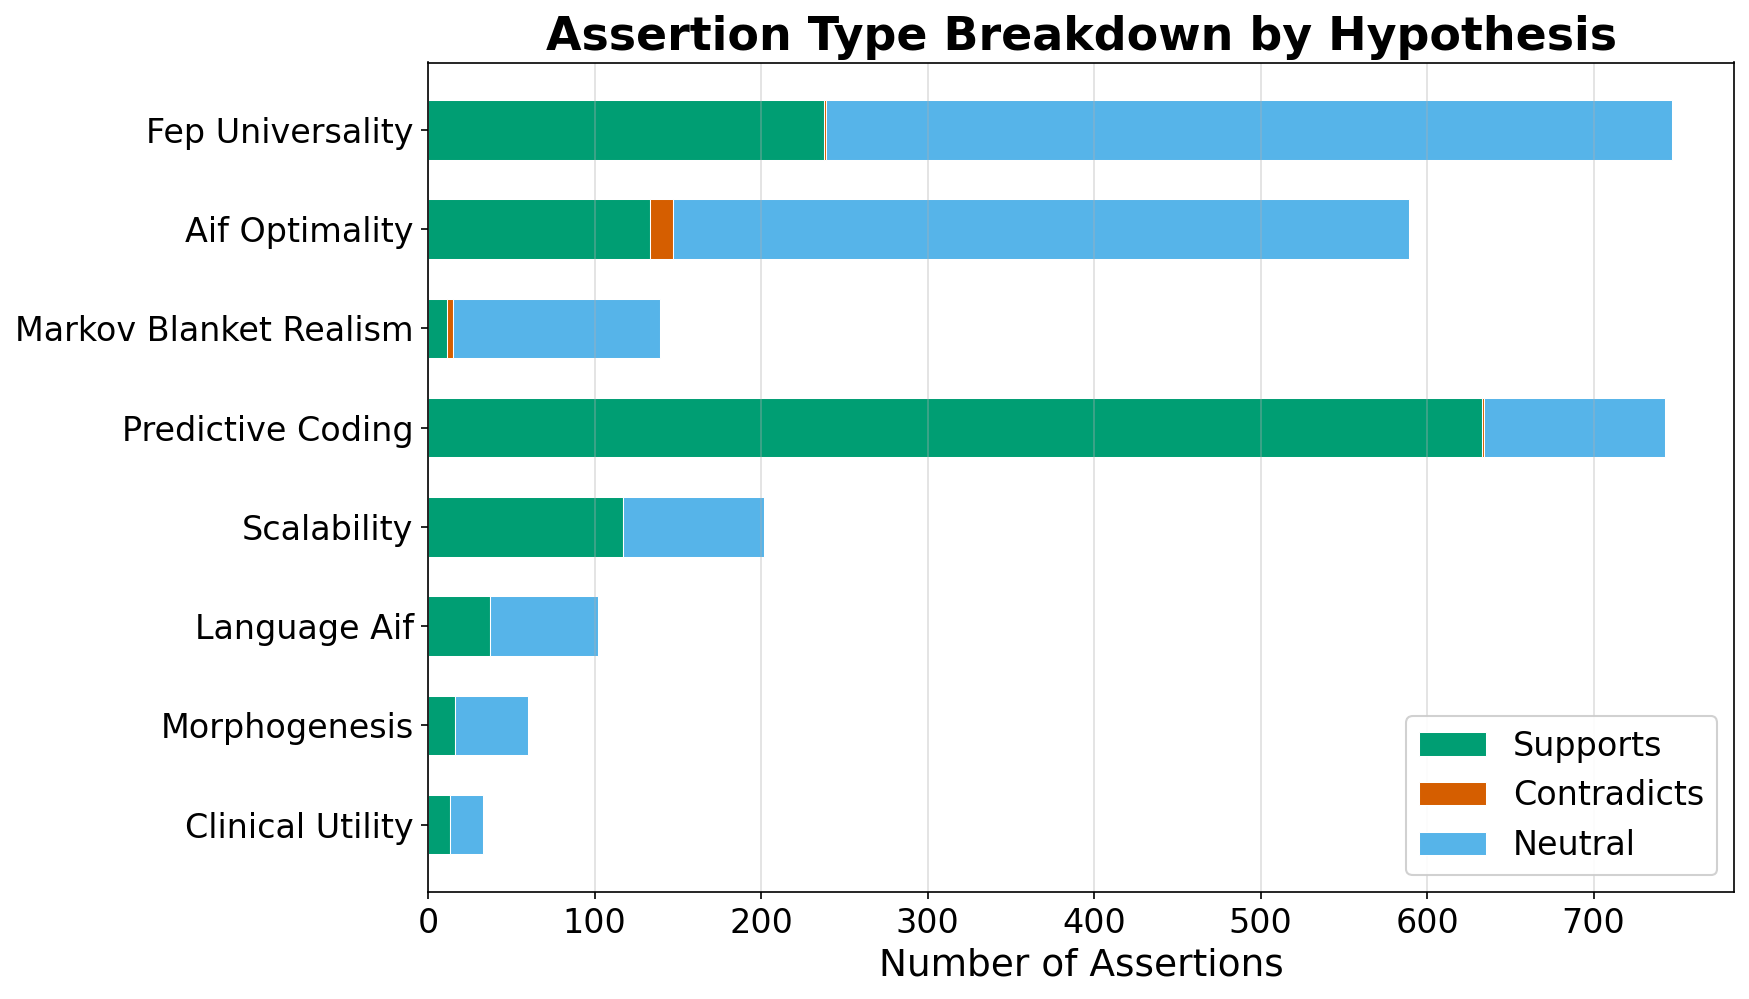
\includegraphics[width=0.9\textwidth]{../figures/assertion_breakdown.png}
\caption{Stacked horizontal bars decomposing per-hypothesis assertions into supports (green), contradicts (red-orange), and neutral (blue) categories ($N = 2,795$ total assertions). Labels show total count and support percentage. The high support fractions are partially attributable to publication bias and affirmative linguistic framing.}
\label{fig:assertion_breakdown}
\end{figure}

\begin{figure}[htbp]
\centering
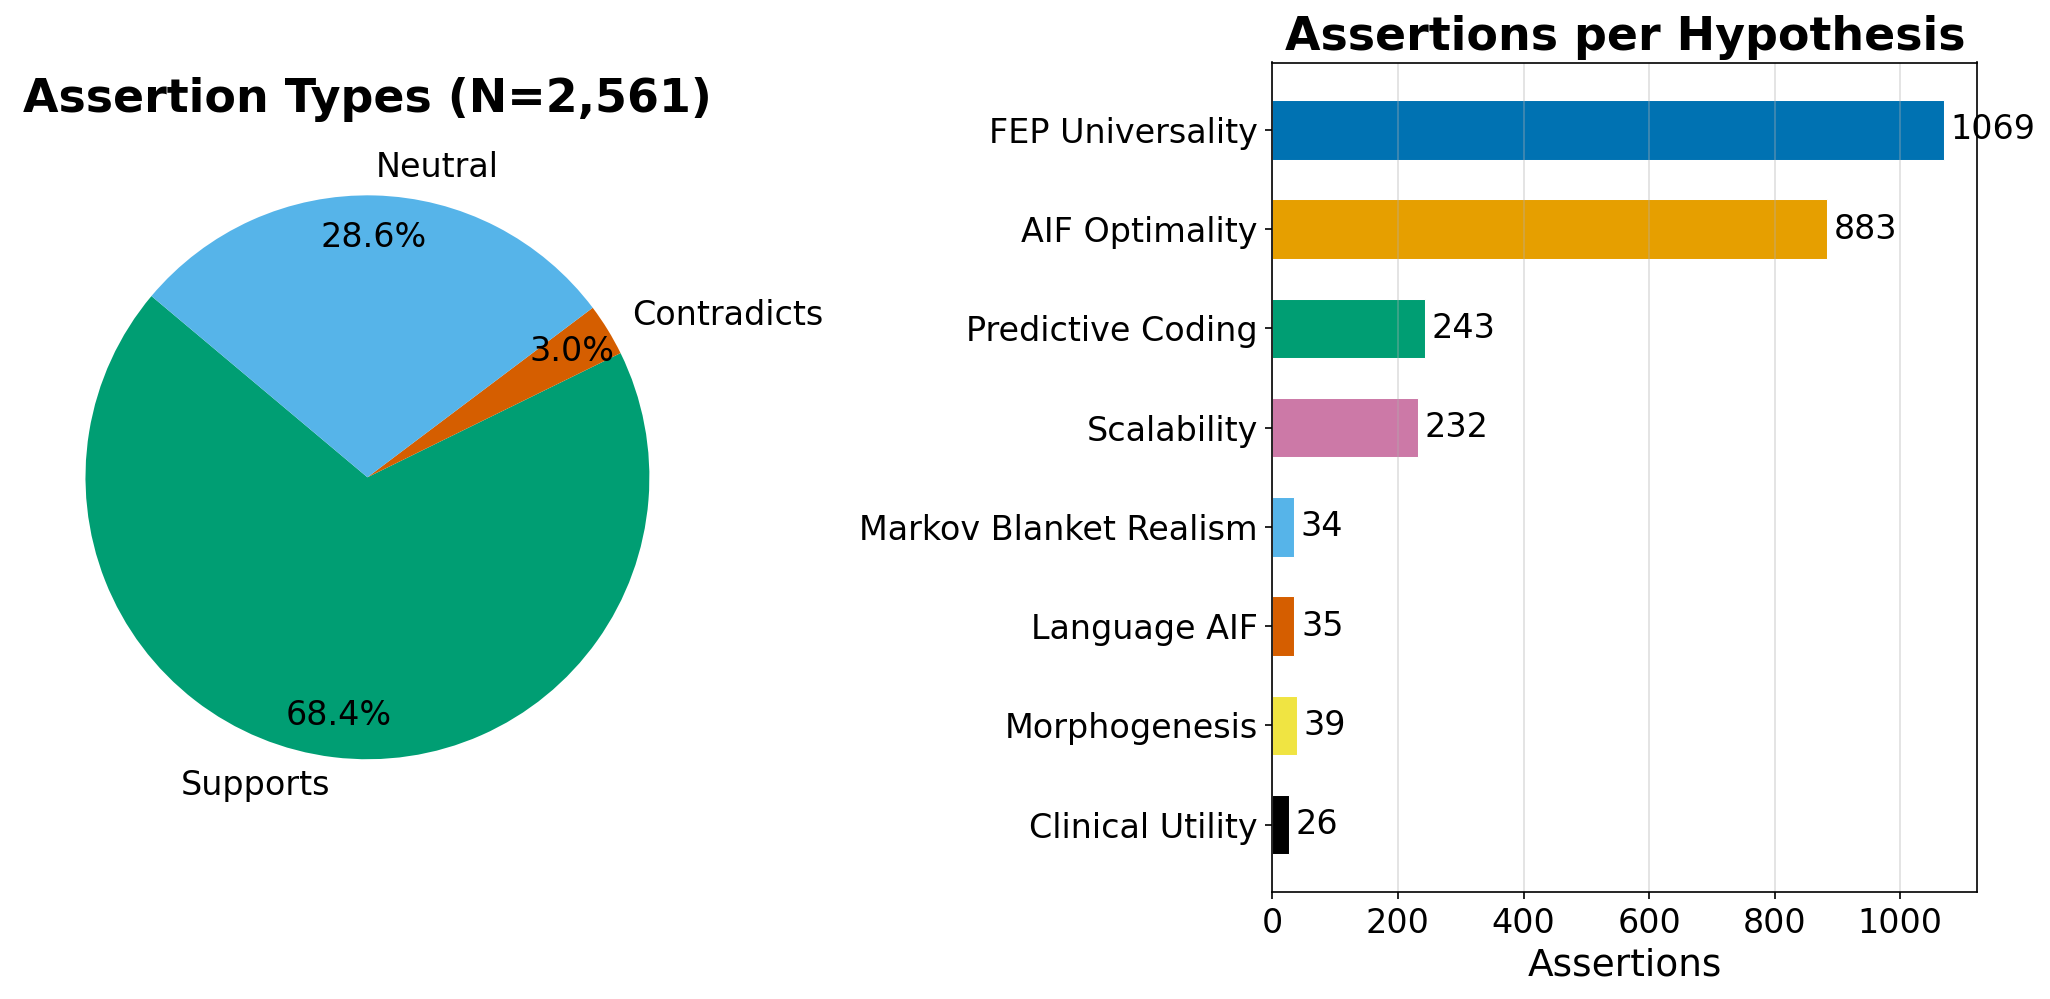
\includegraphics[width=0.9\textwidth]{../figures/assertion_summary.png}
\caption{Multi-panel assertion summary: (left) pie chart of overall assertion type distribution showing supports/contradicts/neutral proportions, (right) per-hypothesis assertion counts with palette-coded bars. $N = 2,795$ assertions extracted from $849$ papers.}
\label{fig:assertion_summary}
\end{figure}
\end{block}

\begin{block}{Limitations of the Current Scoring Approach}
\protect\phantomsection\label{limitations-of-the-current-scoring-approach}
As noted in the \hyperref[sec:methods_kg]{methodology}, these results
reflect a \textbf{tally-based aggregation} of independent LLM-extracted
assertions, weighted by citation count and confidence. This approach
does not account for evidential dependencies (e.g., papers from the same
group testing the same model), does not distinguish between empirical
and theoretical evidence, and treats the LLM's confidence scores as
calibrated probabilities. The assertion counts are also sensitive to
corpus composition: H1's large neutral tally (546) partially reflects
the keyword classifier's tendency to assign papers to the broad A2
(philosophy) category, where FEP universality is implicitly invoked but
rarely explicitly tested. The dominant-neutral pattern for H1 is also
consistent with the falsifiability critique \citep{colombo2021free}: a
principle elastic enough to accommodate any behavior without refutation
will naturally accrue neutral rather than positive or negative
assessments. More sophisticated approaches---including hierarchical
Bayesian models, causal evidence graphs, and evidential diversity
weighting---are discussed as future directions in the
\hyperref[sec:conclusion]{conclusion}.

\begin{block}{Publication Bias and Linguistic Asymmetry
\label{sec:pub_bias}}
\protect\phantomsection\label{publication-bias-and-linguistic-asymmetry}
The predominantly positive scores observed across all eight hypotheses
should be interpreted with two systematic caveats.

First, \textbf{publication bias} systematically inflates supporting
evidence. Academic journals preferentially publish positive and
confirmatory results (\citealt{sterling1959publication}), meaning that
studies finding null or contradictory outcomes for any hypothesis are
less likely to appear in the retrievable literature. This
\textit{file-drawer effect} is well-documented across scientific
disciplines and is expected to disproportionately suppress contradicting
assertions in our extraction pipeline. The Active Inference literature
is particularly susceptible: as a theoretical framework with strong
foundational proponents, papers are more likely to frame results as
consistent with the FEP than as challenges to it.

Second, \textbf{linguistic asymmetry} in academic writing further skews
extraction toward positive classifications. Declarative scholarly claims
are inherently phrased affirmatively---authors write
\texttt{our\ results\ support,\textquotesingle{}\textquotesingle{}}consistent
with,'\,' or
\texttt{extends\ the\ prediction\ of\textquotesingle{}\textquotesingle{}\ far\ more\ frequently\ than}our
results refute'\,' or
\texttt{contradicts\ the\ claim\ that.\textquotesingle{}\textquotesingle{}\ Because\ the\ LLM\ extraction\ pipeline\ operates\ on\ abstract\ text,\ this\ linguistic\ imbalance\ propagates\ directly\ into\ the\ assertion\ distribution.\ Even\ papers\ presenting\ genuinely\ mixed\ evidence\ tend\ to\ frame\ their\ abstracts\ in\ terms\ of\ what\ \textbackslash{}textit\{was\}\ found\ rather\ than\ what\ was\ not,\ biasing\ the\ extracted\ direction\ toward}supports.'\,'

These two effects act in concert: publication bias reduces the number of
contradicting papers in the corpus, and linguistic framing reduces the
number of contradicting assertions extracted from the papers that do
appear. Consequently, the absolute values of hypothesis scores should
not be taken as unbiased measures of scientific consensus. The
\textit{relative} ordering and temporal \textit{trajectories} of
hypothesis scores are more robust indicators, as these biases affect all
hypotheses approximately equally.
\end{block}
\end{block}
\end{frame}

\end{document}
